\clearpage
\subsubsection{逐点排除法}
\label{subsubsec:lab4-task1-point-exclusion}

\paragraph{实验过程与关键代码}

逐点排除法先找出表中所有取值为0的位置，组成非法点列表\texttt{forbidden}。模型只设置8个原始二进制变量，然后对每个非法点添加一条排除不等式。由于LAT中正值和负值都属于合法表项，这里统一使用\texttt{table[a][b] == 0}提取非法点。

对于非法点$q$，当$q_j=0$时，$z_j$表示当前点在第$j$位是否与它不同；当$q_j=1$时，则由$1-z_j$表示。因此，将这8项相加并要求结果至少为1，就能保证当前点至少有一位不同于$q$。实现代码如下：
\begin{lstlisting}
forbidden = [(a, b) for a in range(SIZE) for b in range(SIZE)
             if table[a][b] == 0]
z = model.addVars(8, vtype=gp.GRB.BINARY, name="z")

for point in forbidden:
    q = bits(*point)
    model.addConstr(gp.quicksum(
        z[j] if q[j] == 0 else 1 - z[j]
        for j in range(8)
    ) >= 1)
\end{lstlisting}

每条不等式只排除对应的一个非法二进制点。添加全部约束后，剩余可行点就是表中的非零位置，再由Gurobi按统一参数进行枚举。

\paragraph{实验结果与分析}

代码运行结果如图~\ref{fig:lab4-task1-point-exclusion}所示。
\begin{figure}[H]
    \centering
    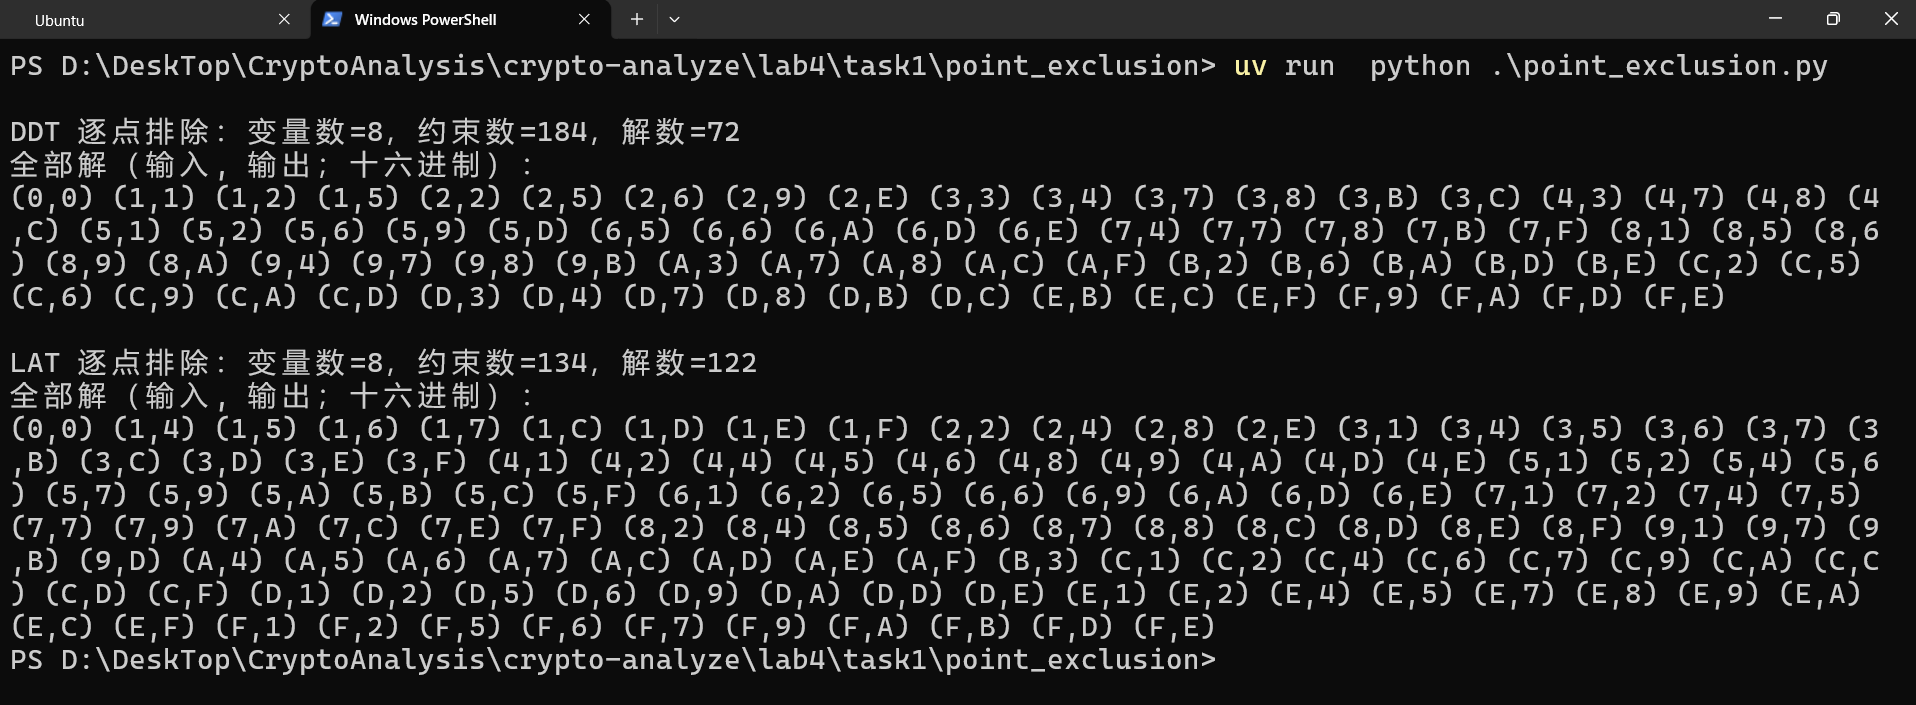
\includegraphics[width=\textwidth]{figures/task1/Grubio_solve_point_exclusion.png}
    \caption{逐点排除法的DDT、LAT模型全解枚举结果}
    \label{fig:lab4-task1-point-exclusion}
\end{figure}

输入、输出各有16种取值，因此共有$16\times16=256$个候选点。DDT中有72个合法点，需要排除$256-72=184$个点，对应184条不等式；LAT中有122个合法点，需要排除$256-122=134$个点，对应134条不等式。两种模型均只有8个二进制变量，与程序输出一致。

枚举得到72个差分合法点和122个线性合法点，具体输入输出对与one-hot法及原始表的非零位置完全一致。该方法保持8个原始变量，通过184条或134条不等式逐点排除非法点，实现了相同的传播关系。
